\documentclass[a4paper,12pt]{article} % тип документа

% Поля страниц
\usepackage[left=2.5cm,right=2.5cm,
    top=2cm,bottom=2cm,bindingoffset=0cm]{geometry}
    
%Пакет дял таблиц   
\usepackage{multirow} 
    
%Отступ после заголовка    
\usepackage{indentfirst}


% Рисунки
\usepackage{floatrow,graphicx,calc}
\usepackage{wrapfig}

%%% Работа с картинками
\usepackage{graphicx}  % Для вставки рисунков
\graphicspath{{images/}{images2/}}  % папки с картинками
\setlength\fboxsep{3pt} % Отступ рамки \fbox{} от рисунка
\setlength\fboxrule{1pt} % Толщина линий рамки \fbox{}
\usepackage{wrapfig} % Обтекание рисунков и таблиц текстом

% Создаёем новый разделитель
\DeclareFloatSeparators{mysep}{\hspace{1cm}}

% Ссылки?
\usepackage{hyperref}
\usepackage[rgb]{xcolor}
\hypersetup{				% Гиперссылки
    colorlinks=true,       	% false: ссылки в рамках
	urlcolor=blue          % на URL
}


%  Русский язык
\usepackage[T2A]{fontenc}			% кодировка
\usepackage[utf8]{inputenc}			% кодировка исходного текста
\usepackage[english,russian]{babel}	% локализация и переносы


% Математика
\usepackage{amsmath,amsfonts,amssymb,amsthm,mathtools}

%%% Дополнительная работа с математикой
\usepackage{amsmath,amsfonts,amssymb,amsthm,mathtools} % AMS
\usepackage{icomma} % "Умная" запятая: $0,2$ --- число, $0, 2$ --- перечисление


% Что-то 
\usepackage{wasysym}


\begin{document}
\begin{center}
	\footnotesize{ФЕДЕРАЛЬНОЕ ГОСУДАРСТВЕННОЕ АВТОНОМНОЕ ОБРАЗОВАТЕЛЬНОЕ 			УЧРЕЖДЕНИЕ ВЫСШЕГО ОБРАЗОВАНИЯ}\\
	\footnotesize{МОСКОВСКИЙ ФИЗИКО-ТЕХНИЧЕСКИЙ ИНСТИТУТ\\(НАЦИОНАЛЬНЫЙ 			ИССЛЕДОВАТЕЛЬСКИЙ УНИВЕРСИТЕТ)}\\
	\footnotesize{ФАКУЛЬТЕТ ОБЩЕЙ И ПРИКЛАДНОЙ ФИЗИКИ\\}
	\hfill \break
	\hfill \break
	\hfill \break
	\hfill \break
\end{center}


\begin{figure*}[h]
    \centering
    \includegraphics*[width=10cm,height=7cm,keepaspectratio]{mipt_eng_text_png.png}
    \label{fig:my_label}
\end{figure*}


\begin{center}   
    \hfill \break
	\hfill \break
	\hfill \break
	\hfill \break
	\large{Лабораторная работа № 2.4.1\\\textbf{Определение теплоты испарения жидкости}}\\
	\hfill \break
	\hfill \break
	\hfill \break
	\hfill \break
	\begin{flushright}
		Баранов Даниил\\
		Группа Б02-103
	\end{flushright}
	\hfill \break
	\hfill \break
	\hfill \break
\end{center}
\hfill \break
\hfill \break
\hfill \break
\hfill \break
\begin{center}
	Долгопрудный, 2022 г.
\end{center}
\thispagestyle{empty}
\newpage
	\textbf{Цель работы:} 1) измерение давления насыщенного пара жидкости при разной температуре; 2) вычисление по полученным данным теплоты испарения с помощью уравения Клапейрона-Клаузиуса.
	\hfill \break
	
	\textbf{В работе используются:} термостат, герметический сосуд, заполненный водой, отсчетный микроскоп.
	
\section{Теоретическое введение}
\subsection*{Уравение Клапейрона-Клаузиуса}

Испарением называется переход вещества из жидкого в газообразное состояние. Оно происходит на свободной поверхности жидкости. При испарении с поверхности вылетают молекулы, образуя над ней пар. Для выхода из жидкости молекулы должны преодолеть силы молекулярного сцепления. Кроме того, при испарении совершается работа против внешнего давления $P$, поскольку объем жидкости меньше объема пара. Не все молекулы жидкости способны совершить эту работу, а только те из них, которые обладают достаточной кинетической энергией. Поэтому переход части молекул в пар приводит к обеднению жидкости быстрыми молекулами, т. е. к ее охлаждению. Чтобы испарение проходило без изменения температуры, к жидкости нужно подводить тепло. Количество теплоты, необходимое для изотермического испарения одного моля жидкости при внешнем давлении, равном упругости ее насыщенных паров, называется молярной теплотой испарения (парообразования).
    
Около тройной точки теплота сублимации $q_s$ равна сумме теплоты плавления $q_m$ и испарения $q_e$, поэтому кривая сублимации идет круче, чем линия испарения:
Теплоту парообразования жидкостей можно измерить непосредственно при помощи калориметра. Такой метод, однако, не позволяет получить точных результатов из-за неконтролируемых потерь тепла, которые трудно сделать малыми. В настоящей работе для определения теплоты испарения применен косвенный метод, основанный на формуле Клапейрона-Клаузиуса:
\begin{equation}
    \label{Klap}
    \frac{dP}{dT} = \frac{L}{T(V_2 - V_1)}
\end{equation}
\break

Здесь $P$ -- давление насыщенного пара жидкости при температуре $T$, $T$ -- абсолютная температура жидкости и пара, $L$ — теплота испарения жидкости, $V_2$ -- объем пара, $V_1$ -- объем жидкости. Найдя из опыта $dP/dT$, $T$, $V_2$ и $V_1$, можно определить $L$ путем расчета. Величины $L$, $V_2$ и $V_1$ в формуле (\ref{Klap}) должны относиться к одному и тому же количеству вещества; мы будем относить их к одному молю.

Из таблицы (\ref{data}) видно, что величина $V_1$ не превышает 0,5\%  от $V_2$. Для нашей точности эксперимента этой величиной можно пренебречь.

Обратимся теперь к $V_2$, которое в дальнейшем будем обозначать $V$. Объем $V$ связан с давелнием и темературой уравнением Ван-дер-Ваальса:

\begin{equation}
    \label{Van-der}
    \left( P + \frac{a}{V^2}\right)(V - b) = RT
\end{equation}
\break

Из рассмотрения таблицы (\ref{data}) следует, что $b$ одного порядка с $V_1$. В уравнении Ван-дер-Ваальса величиной $b$ следует пренебречь. Пренебрежение членом $a/V^2$ по сравнению с $P$ вносит ошибку менее 3\%. При давлении ниже атмосферного ошибки становятся еще меньше. Таким образом, при давлениях ниже атмосферного уравнение Ван-дер-Ваальса для насыщенного пара мало отличается от уравнения Клапейрона. Положим поэтому

\begin{equation}
    \label{ideal}
    P = \frac{RT}{V}
\end{equation}
\break

Подставляя (\ref{ideal}) в (\ref{Klap}) и разрешая уравение относительно $L$, получаем:

\begin{equation}
    \label{L}
    L = \frac{RT^2}{P}\frac{dP}{dT} = -R\frac{d(\mbox{ln }P)}{d(1/T)}
\end{equation}
\break

Эта формула является окончательной.

В нашем эксперименте температура жидкости определяется термометром, давление пара определяется с помощью манометра, а производные  $dP/dT$ и $d(\mbox{ln }P)/ d(1/T)$ можно найти из углового коэффициента касательной к графику  $P(T)$ или как коэффициент наклона прямой на графике с осями ln $P$ и $1/T$.

\section{Экспериментальная установка}

Схема установки изображена на рисунке 1. Наполненный водой резервуар 1 играет роль термостата. Нагревание термостата производится спиралью 2, подогреваемой электрическим током. Для охлаждения воды в термостате через змеевик 3 пропускается водопроводная вода. Вода в термостате перемешивается воздухом, поступающим через трубку 4. Температура воды измеряется термометром 5. В термостат погружен запаянный прибор 6 с исследуемой жидкостью. Над ней находится насыщенный пар (перед заполнением прибора воздух из него был откачан).
Давление насыщенного пара определяется по ртутному манометру,соединенному с исследуемым объемом. Отсчет показаний манометра производится при помощи микроскопа.



\section{Результаты измерений}

Здесь и далее плотность ртути $\rho_q = 13600$ кг/м$^3$. Давление расчитывается по формуле $P = 2\rho g\Delta h$, где $\Delta h = h_2 - h_1$ -- измеренная разность высот столбов ртути.
\break

     


Погрешность рассчёта давления составила $\varepsilon_P \approx 3\%$. Погрешность же измерения температуры составляет не более 1\%.

Графики зависимости давления от температуры представлены на Рис.\ref{fig:temppress} и Рис.\ref{fig:temppressnorm} .



Из графика \ref{fig:temppress} хорошо видно, что зависимость не является линейной. По наклону построеных графиком можем оценить величину $L$ и погрешность её определения. При нагревании она составила $\displaystyle L_H = 42 \pm 1,5 \frac{\mbox{кДж}}{\mbox{моль}}$. При охлаждении теплота испарения составила $\displaystyle L_O = 41 \pm 1,7 \frac{\mbox{кДж}}{\mbox{моль}}$. Погрешности взяты из ошибок в определении коэффициентов фитирующих прямых с помощью МНК. Заметим, что полученные результаты совпадают в пределах погрешности с теоретическим значением $\displaystyle L_O = 40,7 \frac{\mbox{кДж}}{\mbox{моль}}$.

\section{Приложение}

\begin{figure}

    \label{machine}
	\center{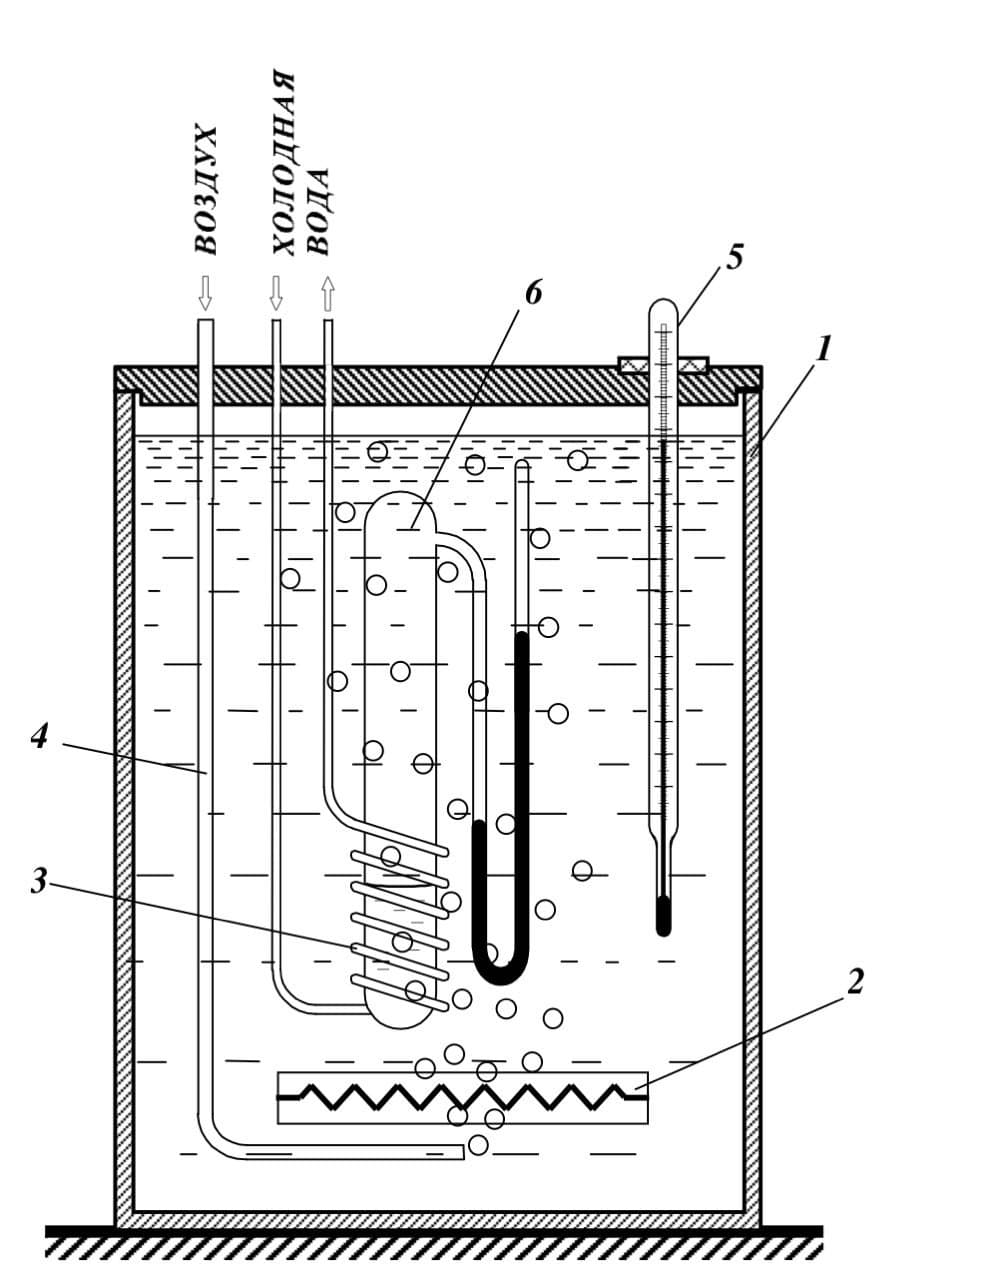
\includegraphics[scale=0.2]{2.4.1/ust_2.jpg}}
	\caption{Схема установки для определения теплоты испарения}
\end{figure}

\begin{figure*}[h]
    \centering
    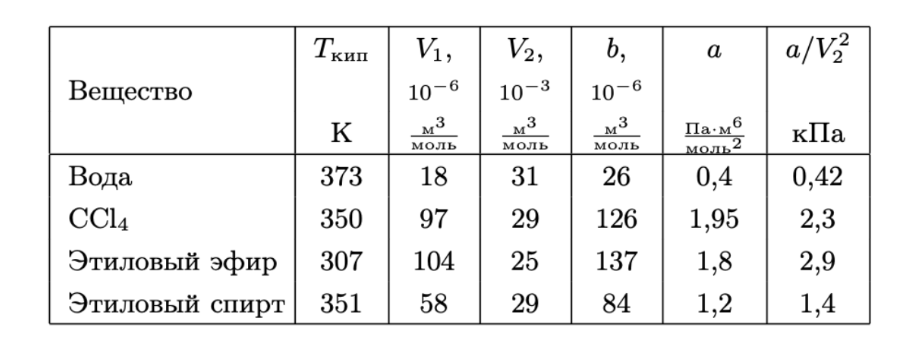
\includegraphics[scale=0.8]{2.4.1/data.PNG}
    \label{data}
\end{figure*}

\begin{table}[h]
    \caption{Начальные измерения}
    \centering
        \begin{tabular}{|c|c|c|c|c|}
     \hline $T_{init}$, $^\circ$C & $h_1$, мм & $h_2$, мм & $\delta h$, мм & $P_{init}$, Па \\
    \hline 21,3 & 72,6 & 93,5 & 20,9 & 2788 \\
    \hline

\end{tabular}

    \label{tab:init}
\end{table}
\begin{table}[h]
    \caption{Измерения при нагреве}
    \begin{tabular}{|c|c|c|}
        \hline $T$, $^\circ C$  &  \Delta h, мм & $P$, Па \\
        \hline 24,0 & 22,7 & 3087 \\
        \hline 27,0 & 26,7 & 3631 \\
        \hline 30,0 & 31,5 & 4284 \\
        \hline 33,0 & 36,5 & 4964 \\
        \hline 36,0 & 43,3 & 5889 \\
        \hline 39,0 & 50,3 & 6841 \\
        \hline 42,0 & 58,5 & 7956 \\
        \hline 45,0 & 68,9 & 9370 \\
        \hline 48,0 & 79,1 & 10758 \\
        \hline 50,0 & 88,9 & 12090 \\
        \hline
        
    \end{tabular}

    \label{tab:my_label}
\end{table}
\begin{table}[h]
    \caption{Измерения при охлаждении}
    \begin{tabular}{|c|c|c|}
        \hline $T$, $^\circ C$  &  \Delta h, мм & $P$, Па \\
        \hline 45,9 & 74,1 & 10078 \\
        \hline 43,0 & 63,9 & 8690 \\
        \hline 40,0 & 54,9 & 7466 \\
        \hline 37,0 & 46,9 & 6378 \\
        \hline 34,0 & 40,3 & 5481 \\
        \hline 31,0 & 34,3 & 4665 \\
        \hline 28,0 & 28,9 & 3930 \\
        \hline 25,0 & 24,3 & 3305 \\
        \hline
        
    \end{tabular}

    \label{tab:my_label}
\end{table}

\begin{figure}[h]
    \centering
    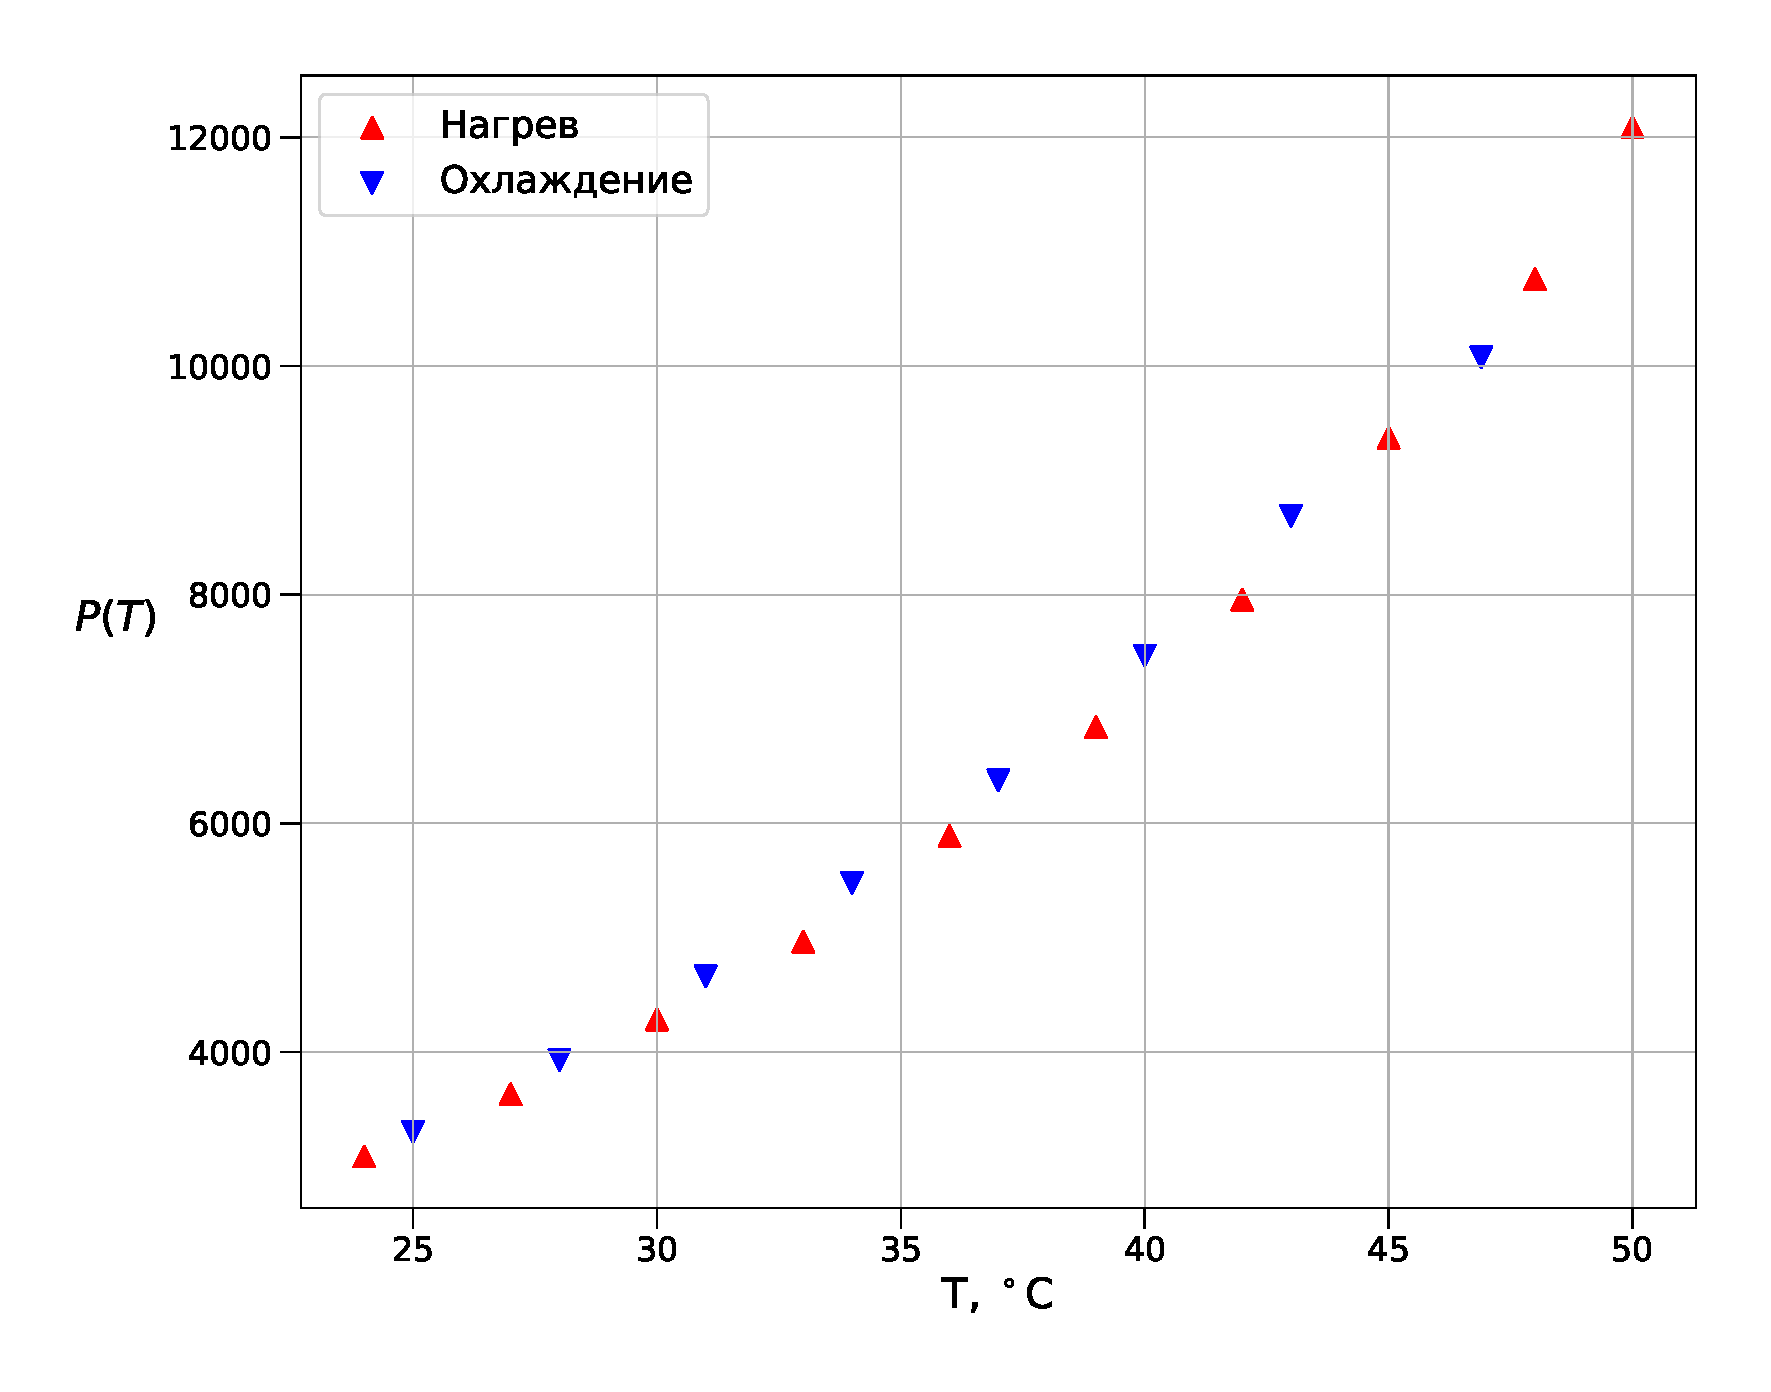
\includegraphics[scale = 0.55]{2.4.1/temppress.pdf}
    \caption{Зависимость $P(T)$}
    \label{fig:temppress}
\end{figure}

\begin{figure}[h]
    \centering
    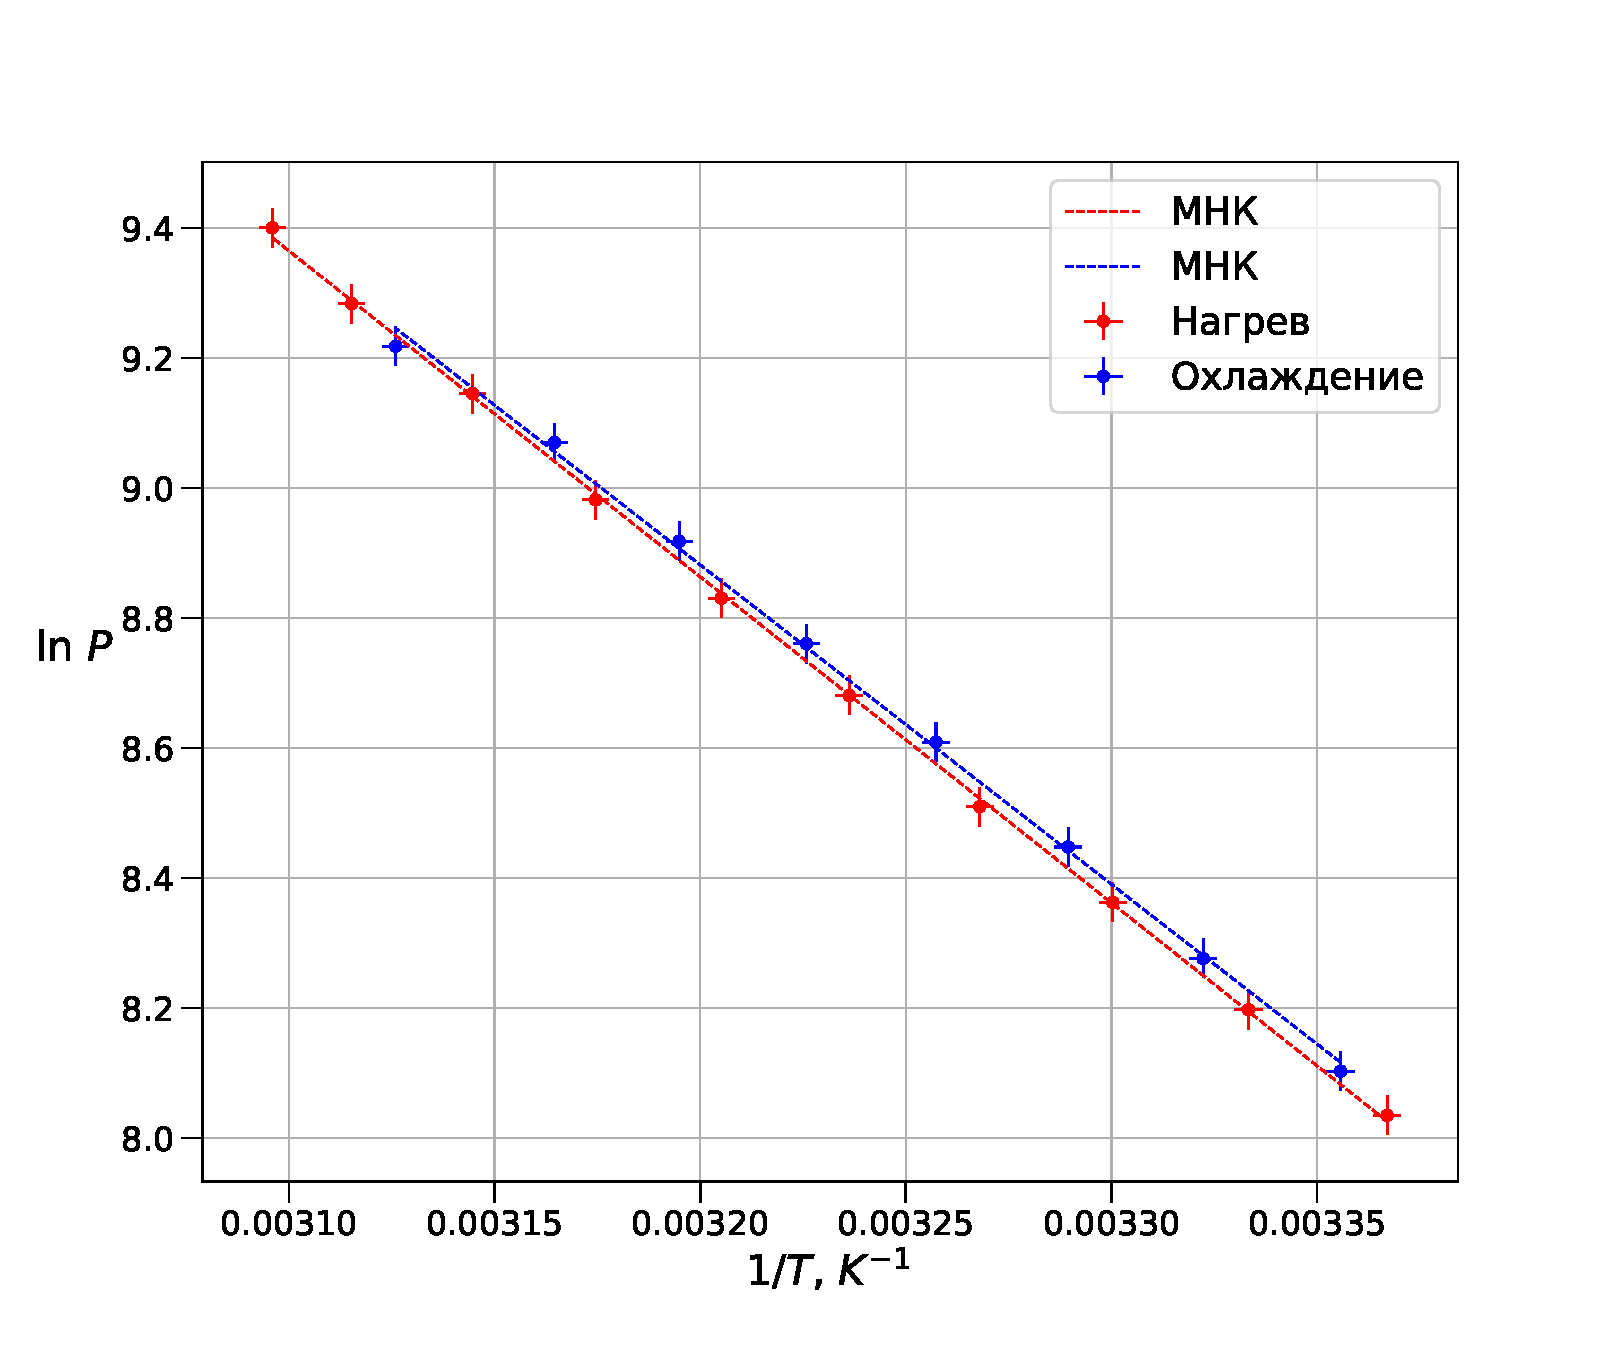
\includegraphics[scale = 0.6]{2.4.1/lnPT.pdf}
    \caption{Зависимость ln $P$ от $1/T$}
    \label{fig:temppressnorm}
\end{figure}





\end{document}
